
\begin{figure}[t]
    \centering
    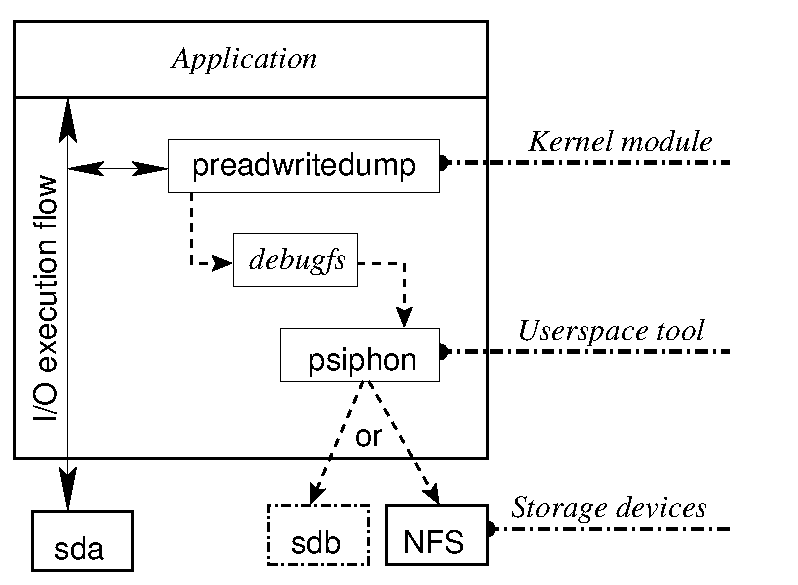
\includegraphics[scale=0.8]{tracingchap-figures/toolkit-usability.pdf}
%    \vspace{-0.1in}
    \caption{Toolkit usage: \textit{Figure shows the data flow
			for the trace collection, from the kernel module to \texttt{debugfs}
		and then to either NFS or another local storage device.}}
    \label{fig:toolkit-usability}
%    \vspace{-0.2in}
\end{figure}

There are primarily three tools in our trace generation toolkit, as listed
below. The first two are both kernel modules, with a slight difference 
in the \texttt{jprobe} handlers used in each, whereas the third one is
a userspace tool.
\begin{enumerate}
	\item \texttt{pdatadump}: For every block write request, this kernel
		module dumps the written content as well as other identifying 
		information like sector address, major number, minor number, etc.
		For every read request, only the identifying information is 
		output, and the data content itself is not dumped.
	\item \texttt{preadwritedump}: Similar to \texttt{pdatadump}, with the
		only difference that data content is dumped for read requests as 
		well, in addition to write requests.
	\item \texttt{psiphon}: This is the userspace tool that can siphon 
		logs written in the \texttt{debugfs} files, into regular files.
		High-speed transfer is achieved using \texttt{mmap} of the
		regular files. This is a generic tool, in the sense that it can 
		be used to transfer logs from \texttt{debugfs} filesystem into
		the regular filesystem for any files, provided the filenames 
		are provided as input. Thus, it can be used in tandem with any
		kernel module that dumps output into the \texttt{debugfs} filesystem.
\end{enumerate}

\paragraph{Usability of the toolkit.}
The \texttt{pdatadump}, \texttt{preadwritedump} and the \texttt{psiphon}
tools can be used within any linux machine (both physical or virtual),
and can be used to trace the block read and write requests for any 
specified device (namely, \texttt{/dev/sda}, \texttt{/dev/sdb}, etc)
or even for a specific hard-disk partition (namely, 
\texttt{/dev/sda1}, \texttt{/dev/sda2} and so on). 

\paragraph{Measures to avoid the problem of \textit{recursive tracing}.}
When the \texttt{psiphon} tool transfers the trace data from 
\texttt{debugfs} filesystem into regular files, if the destination file
is on the same disk/partition as the one being traced, it can 
result in ``recursive tracing''\textemdash{}traces that are being output themselves 
getting traced. To avoid such a scenario, we prefer the usage of a separate
network-attached (i.e. remote storage, eg. NFS) storage as the destination 
file system for \texttt{psiphon} output files. 
This option is built into the installation script for
the tracing toolkit. Although it is possible to use local storage also 
for log collection, it should be ensured that the specified partitions/devices
for tracing and log collection are distinct, to avoid the 
``recursive tracing'' issue.


Fig. \ref{fig:toolkit-usability} shows ways in which the tracing toolkit
can be used in both physical and virtual machines. Physical machines may 
potentially have multiple hard-disks, so choosing one for tracing and
another for log collection is a possibility. However, typical virtual
machines are created with a single partition, by default. In this case,
creating an NFS partition to be used for log collection is a
straight-forward choice.

